\documentclass{article}
\usepackage[utf8]{inputenc}
\usepackage{amsmath, amssymb, amsthm}
\usepackage[margin=0.5in]{geometry}
\usepackage{graphicx}  % For including images
\usepackage{listings}  % For including code
\usepackage{xcolor}  % For code highlighting
\usepackage{subcaption}  % For subfigures
\usepackage{hyperref}
\usepackage{tikz}
\usepackage{pdfpages}
\usetikzlibrary{positioning}

% Define theorem environments
\newtheorem{theorem}{Theorem}
\newtheorem{lemma}{Lemma}
\newtheorem{definition}{Definition}
\newtheorem{corollary}{Corollary}
% Define custom solution environment
\newenvironment{solution}{\noindent\textbf{Solution:} }{\qed}
% Code listing style
\lstset{
    language=Python,
    basicstyle=\ttfamily\footnotesize,
    keywordstyle=\color{blue},
    commentstyle=\color{gray},
    stringstyle=\color{red},
    breaklines=true,
    numbers=left,
    numberstyle=\tiny\color{gray},
    frame=single
}
\usetikzlibrary{positioning, shapes, arrows.meta}

\title{ECE-GY 7123 Advanced Machine Learning \\ \Large Homework 1}
\author{Ali Hamza (ah7072)}
\date{\today}

\begin{document}
\maketitle
\newpage


% Download Cloud and Spambase data set from the UCI repository
% (https://archive.ics.uci.edu/ml/datasets.php). Implement Static Expert and Fixed-Share (alpha)
% algorithms. For Fixed-Share (alpha) algorithm explore 3 different settings of alpha. Use 6 experts in your
% implementation. Your experts can be designed in any way you want to. Make sure to clearly describe
% them. Report the following: i) the evolution of expert weights with iterations, ii) the cumulative loss of
% the learner versus iterations, and iii) the cumulative loss of the experts versus iterations. What
% conclusions can you draw from these experiments? Describe all your observations.

\section*{Problem 1}
\subsection*{(i) Static Expert \& Fixed-Share Algorithms}

In our online aggregation framework, the learner combines the predictions of $N$ experts by maintaining and updating a weight vector 
\[
\mathbf{w}_t = \left( w_{1,t}, \ldots, w_{N,t} \right)
\]
over the experts. At each round $t$, each expert $i$ provides a prediction $\hat{y}_{i,t}$ on the input $x_t$ and incurs a loss $\ell_{i,t}$. The aggregated prediction $\hat{y}_t$ is computed using a weighted majority vote. For binary classification, one common approach is to compute
\[
p_{1,t} = \sum_{i=1}^{N} w_{i,t} \, \mathbf{1}\{\hat{y}_{i,t} = 1\},
\]
and then set
\[
\hat{y}_t = \begin{cases} 
1, & \text{if } p_{1,t} \geq 0.5, \\[1mm]
0, & \text{otherwise.}
\end{cases}
\]

\noindent\textbf{Static Expert Algorithm:} \\
The static expert algorithm updates the weights via the exponential weights rule:
\[
w_{i,t+1} = \frac{w_{i,t} \exp\bigl(-\eta\,\ell_{i,t}\bigr)}{\sum_{j=1}^{N} w_{j,t} \exp\bigl(-\eta\,\ell_{j,t}\bigr)},
\]
where $\eta > 0$ is the learning rate. This update rapidly decreases the weight of experts that incur high loss. However, if an expert’s weight becomes very small, it is difficult for it to recover even if it later becomes accurate.\\

\noindent\textbf{Fixed-Share Algorithm:} \\
To address nonstationarity, the fixed-share algorithm introduces a weight-sharing step that redistributes a fraction $\alpha$ of the weight uniformly among all experts. The update proceeds in two stages:

\begin{enumerate}
    \item \textbf{Exponential Weight Update:} Compute the intermediate weights:
    \[
    \tilde{w}_{i,t+1} = w_{i,t} \exp\bigl(-\eta\,\ell_{i,t}\bigr).
    \]
    
    \item \textbf{Weight Redistribution:} Update the weights with sharing:
    \[
    w_{i,t+1} = (1-\alpha) \, \tilde{w}_{i,t+1} + \alpha \, \frac{1}{N} \sum_{j=1}^{N} \tilde{w}_{j,t+1},
    \]
    and then normalize so that $\sum_{i=1}^{N} w_{i,t+1} = 1$.
\end{enumerate}
Here, $\alpha \in [0,1]$ controls the degree of weight sharing. When $\alpha = 0$, the algorithm reduces to the static expert algorithm. Increasing $\alpha$ maintains diversity among the experts, which is beneficial when the best expert changes over time.


\subsection*{(ii) Experts}
Given that we are dealing with a labeled (\href{https://archive.ics.uci.edu/ml/datasets/spambase}{spambase}) and unlabled dataset (\href{https://archive.ics.uci.edu/ml/datasets/Cloud}{cloud}), we choose to use two sets of experts. The first set of experts is designed for supervised learning, while the second set is unsupervised learning. We use six experts in each set to ensure diversity in our predictions. The experts are designed as follows:
\newpage
\begin{itemize}
  \item \textbf{Supervised Experts:}
  \begin{enumerate}
      \item \textbf{Logistic Regression (Default):} This linear model serves as a strong baseline and is computationally efficient. Its simplicity makes it easy to interpret and provides a reference point for the performance of more complex models.
      \item \textbf{Naive Bayes:} A Gaussian Naive Bayes classifier assumes feature independence and is extremely fast to train. Despite its simplicity, it often performs surprisingly well, especially when the independence assumption holds approximately, offering a probabilistic perspective on the data.
      \item \textbf{RandomForest:} This ensemble method builds multiple decision trees and aggregates their predictions. Random forests are robust to overfitting and capture non-linear relationships in the data, making them a powerful choice for many classification tasks.
      \item \textbf{SVM:} A Support Vector Machine with an RBF kernel is capable of modeling complex, non-linear boundaries. Its use of kernel methods makes it effective in high-dimensional spaces, providing a strong contrast to linear models.
      \item \textbf{MLP:} The Multi-Layer Perceptron is a neural network model that can learn intricate non-linear patterns through its hidden layers. Its flexibility allows it to adapt to complex data structures, complementing the other, more traditional classifiers.
      \item \textbf{GradientBoosting:} This boosting ensemble method iteratively improves its predictions by focusing on the errors of previous models. Gradient boosting is known for its high accuracy and robustness, making it a competitive expert in diverse datasets.
  \end{enumerate}
  
  \item \textbf{Unsupervised Experts:}
  \begin{enumerate}
      \item \textbf{KMeans (2 Clusters):} A simple and effective clustering algorithm that partitions the data into $K$ clusters. KMeans is computationally efficient and scales well to large datasets, making it a popular choice for many clustering tasks.
      \item \textbf{KMeans (3 Clusters):} Similar to the 2-cluster version, this expert partitions the data into 3 clusters, allowing for more complex structures to be captured.
      \item \textbf{KMeans (4 Clusters):} With 4 clusters, this expert can capture even more intricate patterns in the data, providing a richer representation of the underlying structure.
      \item \textbf{Gaussian Mixture Model (2 Components):} A probabilistic clustering method that models the data as a mixture of Gaussians. GMMs are flexible and can capture complex data distributions, making them a powerful tool for clustering tasks.
      \item \textbf{Gaussian Mixture Model (3 Components):} Similar to the 2-component version, this expert models the data as a mixture of 3 Gaussians, allowing for more nuanced representations of the data.
      \item \textbf{Gaussian Mixture Model (4 Components):} With 4 components, this expert can capture even more complex data distributions, providing a detailed view of the underlying data structure.
  \end{enumerate}

\end{itemize}

\subsection*{(iii) Experiments}

We conduct experiments on both the Cloud and Spambase datasets from the UCI repository. The experimental procedure is as follows:

\begin{enumerate}
    \item \textbf{Data Preprocessing:}
    \begin{enumerate}
      \item \textbf{Cloud:} The Cloud dataset is unsupervised and contains 1024 unlabeled instances. We preprocess the data by normalizing each feature to have zero mean and unit variance. We then split the data into training and test sets using an 80-20 split. We use the \texttt{sklearn} \texttt{train\_test\_split} and \texttt{StandardScaler} are used for this purpose.
      \item \textbf{Spambase:} The Spambase dataset is supervised and contains 4601 labeled instances. We preprocess the data by normalizing each feature to have zero mean and unit variance. We then split the data into training and test sets using an 80-20 split. We use the \texttt{sklearn} \texttt{train\_test\_split} and \texttt{StandardScaler} are used for this purpose.
    \end{enumerate}
    \item \textbf{Offline Training:}
    \begin{enumerate}
        \item For the supervised setting, we train each expert on the training data using the default hyperparameters. We use the \texttt{sklearn} implementations of the classifiers for this purpose. We also evaluate the performance of each expert on the test data. The results are shown in Figure \ref{fig:spambase_off}.
        \begin{figure}[ht]
          \centering
          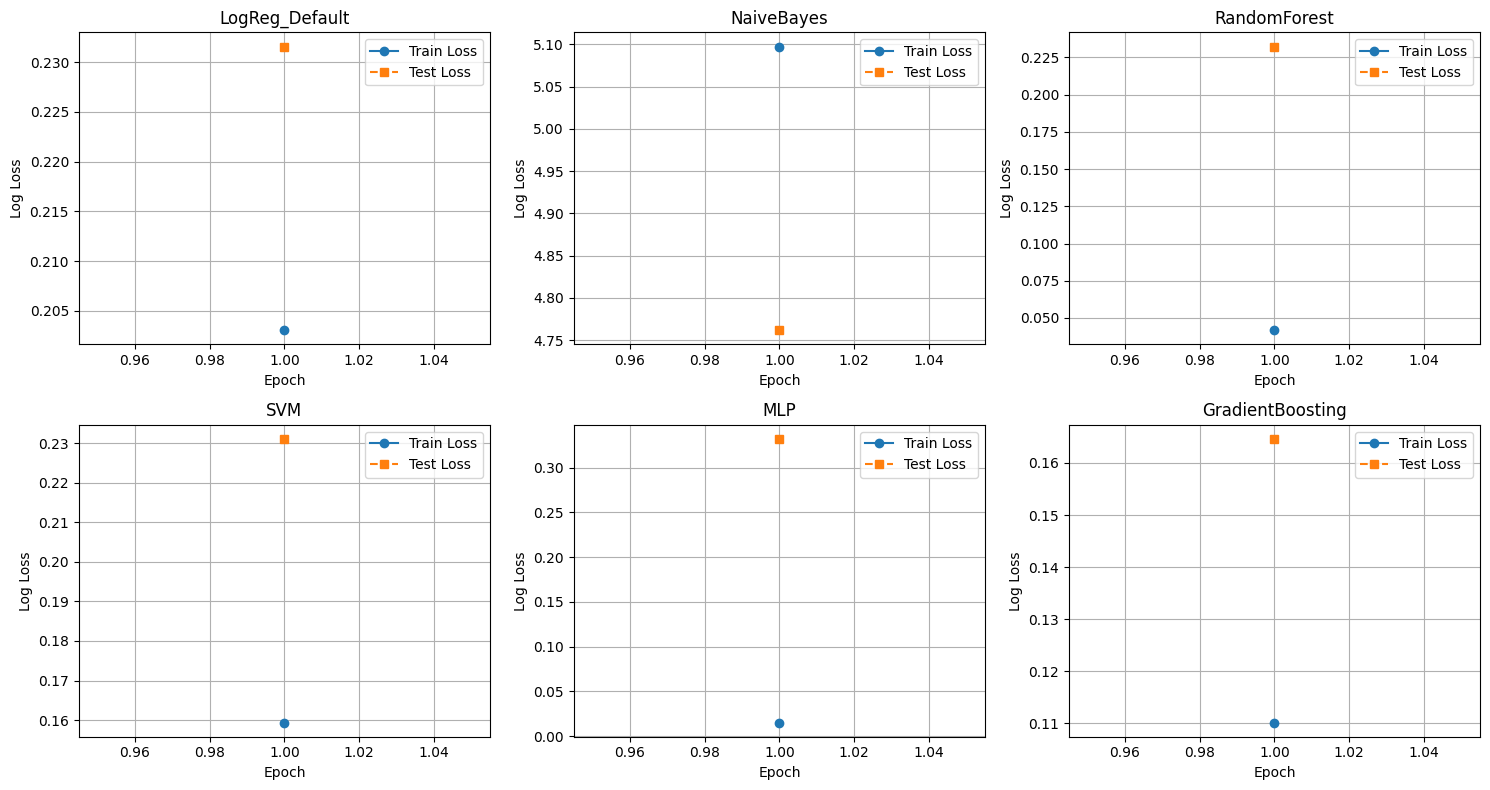
\includegraphics[width=0.6\textwidth]{spambase_off.png}
          \caption{Performance of supervised experts on the Spambase dataset.}
          \label{fig:spambase_off}
        \end{figure}
        \item For the unsupervised setting, we train each expert on the training data using the default hyperparameters. We use the \texttt{sklearn} implementations of the clustering algorithms for this purpose. The clustering results are shown in Figure \ref{fig:cloud_off}.
        \begin{figure}[ht]
          \centering
          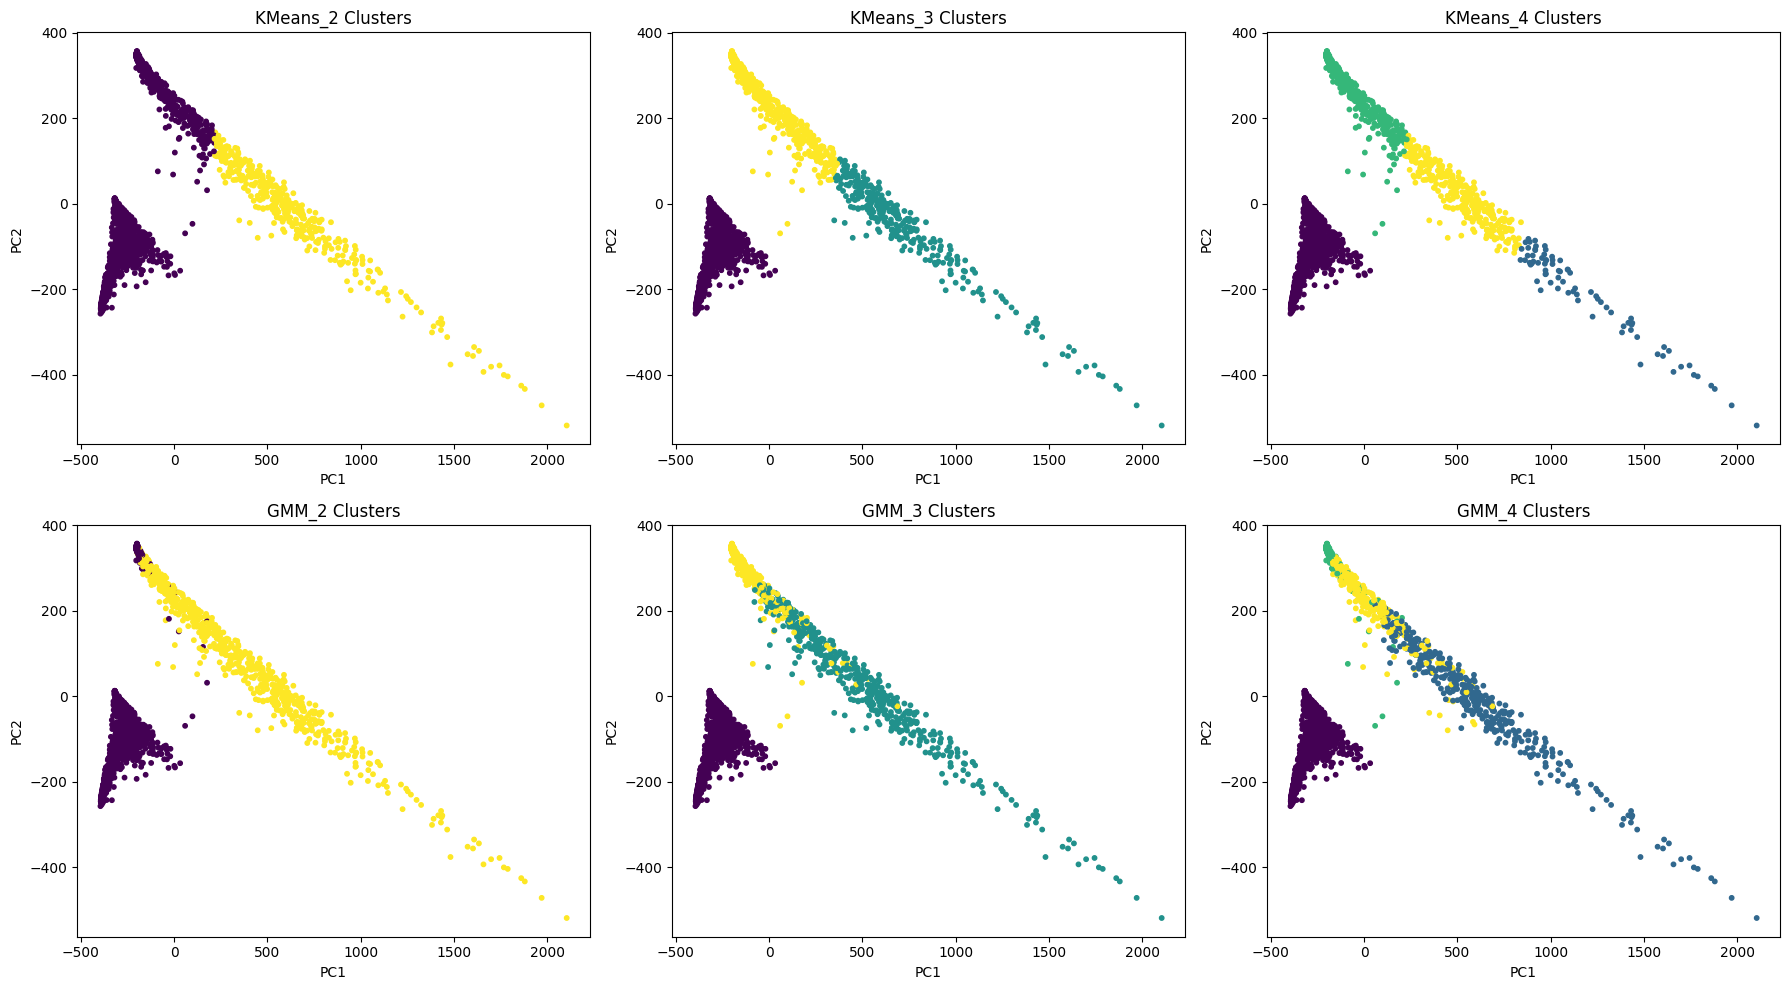
\includegraphics[width=0.6\textwidth]{cloud_off.png}
          \caption{Clustering results of unsupervised experts on the Cloud dataset.}
          \label{fig:cloud_off}
        \end{figure}
    \end{enumerate}
    
    \item \textbf{Online Aggregation:}\\
    The online aggregation algorithm processes the test data sequentially (sample-by-sample). The weight update strategies for both supervised and unsupervised settings make use of either the static expert or fixed-share algorithm. The experts provide predictions on the test data, and the aggregator combines these predictions to make a final decision. The instantaneous loss is calculated for each expert and the aggregator. We explore three different settings of $\alpha$ for the fixed-share algorithm (e.g., $\alpha = 0.01$, $\alpha = 0.1$, and $\alpha = 0.3$).
    \begin{itemize}
        \item \textbf{Static Update:} 
        \[
        w_{i,t+1} = \frac{w_{i,t} \exp\bigl(-\eta\,\ell_{i,t}\bigr)}{\sum_{j=1}^{N} w_{j,t} \exp\bigl(-\eta\,\ell_{j,t}\bigr)},
        \]
        \item \textbf{Fixed-Share Update:} First perform the exponential update, then apply the sharing step:
        \[
        w_{i,t+1} = (1-\alpha) \, \tilde{w}_{i,t+1} + \alpha \, \frac{1}{N} \sum_{j=1}^{N} \tilde{w}_{j,t+1},
        \]
        where $\tilde{w}_{i,t+1} = w_{i,t} \exp\bigl(-\eta\,\ell_{i,t}\bigr)$.
    \end{itemize}
    However, the calculation of loss differs for supervised and unsupervised settings, which are as follows:
    \begin{enumerate}
      \item \textbf{Supervised Loss:} We use the 0-1 loss for the supervised setting, which is defined as:
      \[
      \ell_{i,t} = \begin{cases}
      1, & \text{if } \hat{y}_{i,t} \neq y_t, \\
      0, & \text{otherwise.}
      \end{cases}
      \]
      \begin{itemize}
        \item Each expert produces a prediction $\hat{y}_{i,t}$.
        \item The aggregator computes a weighted majority vote to obtain $\hat{y}_t$, as described above.
        \item The instantaneous loss for each expert and the aggregator is computed using 0--1 loss.
      \end{itemize}
      
      \item \textbf{Unsupervised Loss:} We use the K-means cost as the loss function for the unsupervised setting. The K-means cost is defined as:
      \[
      \ell_{i,t} = \sum_{i=1}^{n} \| x_i - \mu_{c(i)} \|^2,
      \]
      where $\mu_{c(i)}$ is the centroid of the cluster to which $x_i$ is assigned.
      \begin{itemize}
        \item Each expert produces a clustering of the data sample $x_test$.
        \item The aggregator computes the K-means cost for each expert's clustering.
        \item The instantaneous loss for each expert and the aggregator is computed using the K-means cost.
      \end{itemize}
      \end{enumerate}
    
    \item \textbf{Metrics:} \\
    During the online phase, we record:
    \begin{itemize}
        \item \textbf{Evolution of Expert Weights:} The weight vector $\mathbf{w}_t$ after each iteration.
        \item \textbf{Cumulative Loss of the Aggregator:}
        \[
        L_{\text{aggregator}}(T) = \sum_{t=1}^{T} \ell(\hat{y}_t, y_t).
        \]
        \item \textbf{Cumulative Loss of Each Expert:}
        \[
        L_i(T) = \sum_{t=1}^{T} \ell(\hat{y}_{i,t}, y_t).
        \]
    \end{itemize}
    \item \textbf{Visualization and Analysis:} \\
    We plot the 3 metrics for both supervised and unsupervised setting, for both weight update strategies, and for each value of $\alpha$ for the fixed-share algorithm. 
    \begin{enumerate}
      \item Supervised Setting: Figure \ref{fig:supervised_comparison} shows the evolution of expert weights and the cumulative loss on the Spambase dataset.
      \item Unsupervised Setting: Figure \ref{fig:unsupervised_comparison} shows the evolution of expert weights and the cumulative loss on the Cloud dataset.
    \end{enumerate}

    \end{enumerate}
    \begin{figure}[ht]
      \centering
      \begin{subfigure}[b]{0.3\textwidth}
        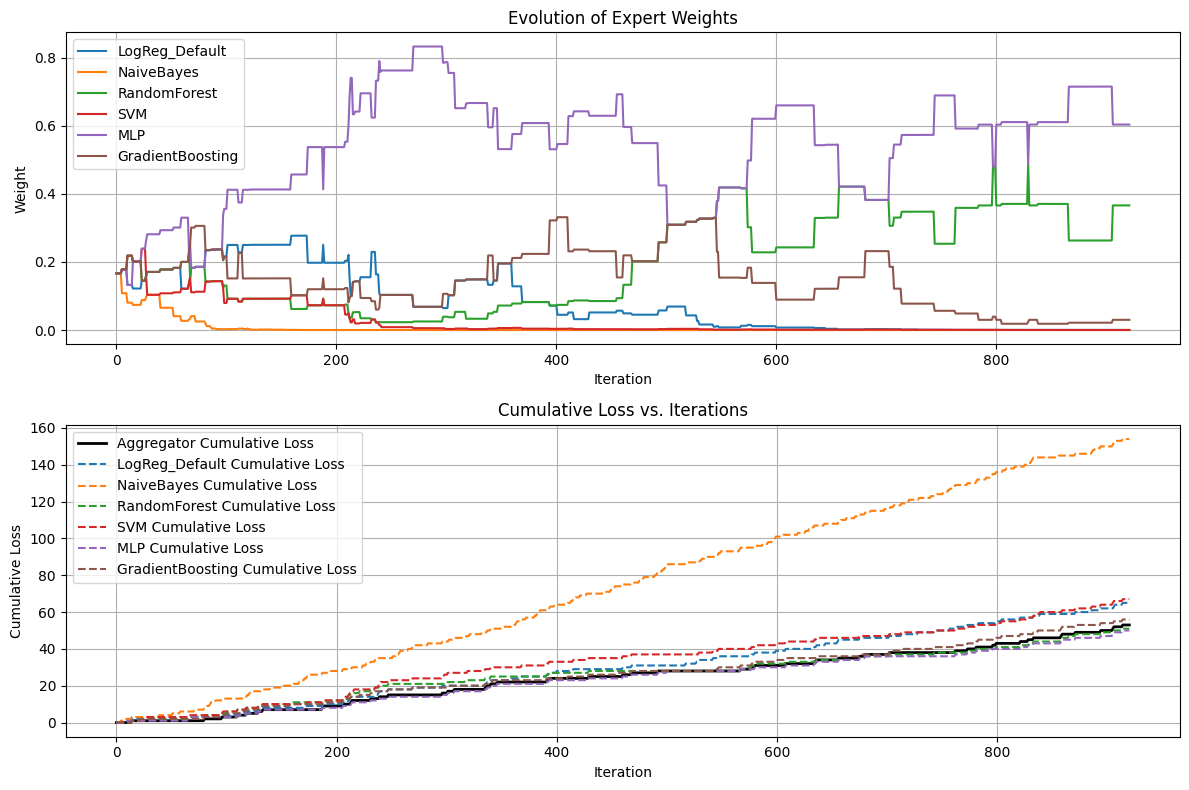
\includegraphics[width=\textwidth]{spambase_static.png}
        \caption{Static Expert}
        \label{fig:supervised_static_weights}
      \end{subfigure}
      \begin{subfigure}[b]{0.3\textwidth}
        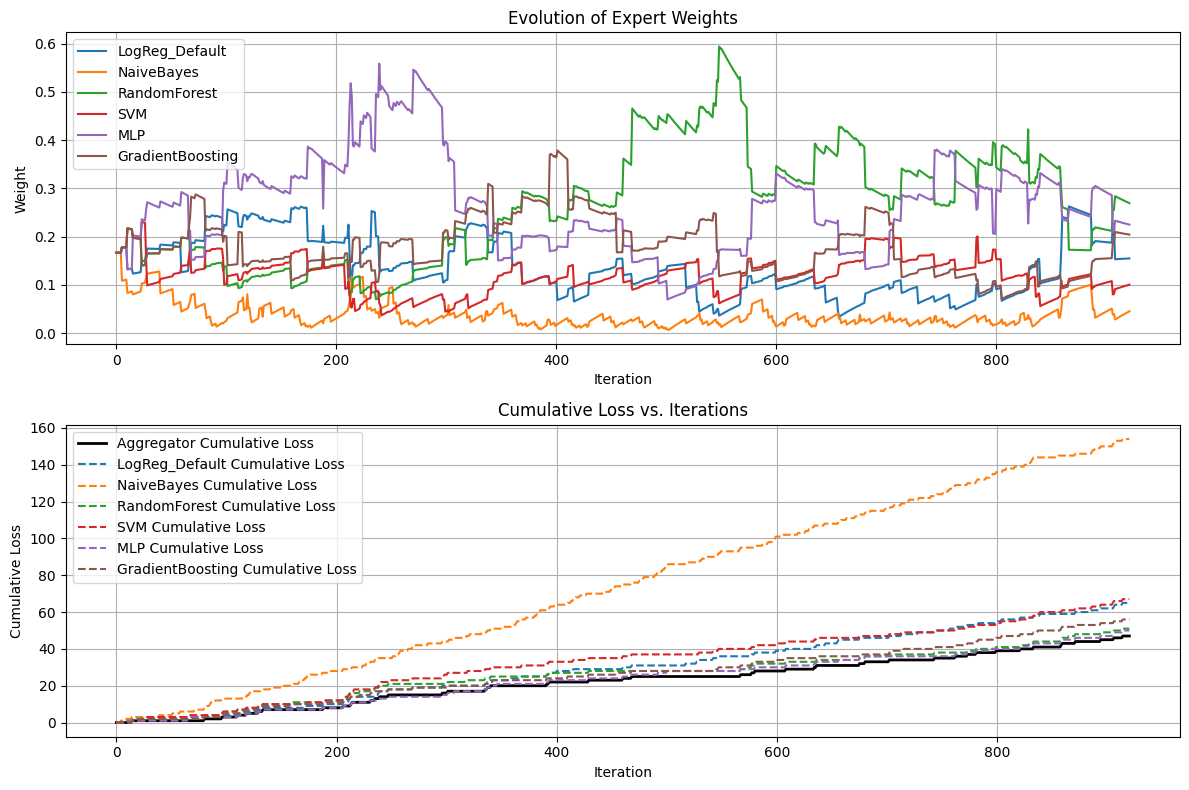
\includegraphics[width=\textwidth]{spambase_fixed_0.01.png}
        \caption{Fixed-Share ($\alpha = 0.01$)}
        \label{fig:supervised_fixed_share_weights_0.01}
      \end{subfigure}
      \\
      \begin{subfigure}[b]{0.3\textwidth}
        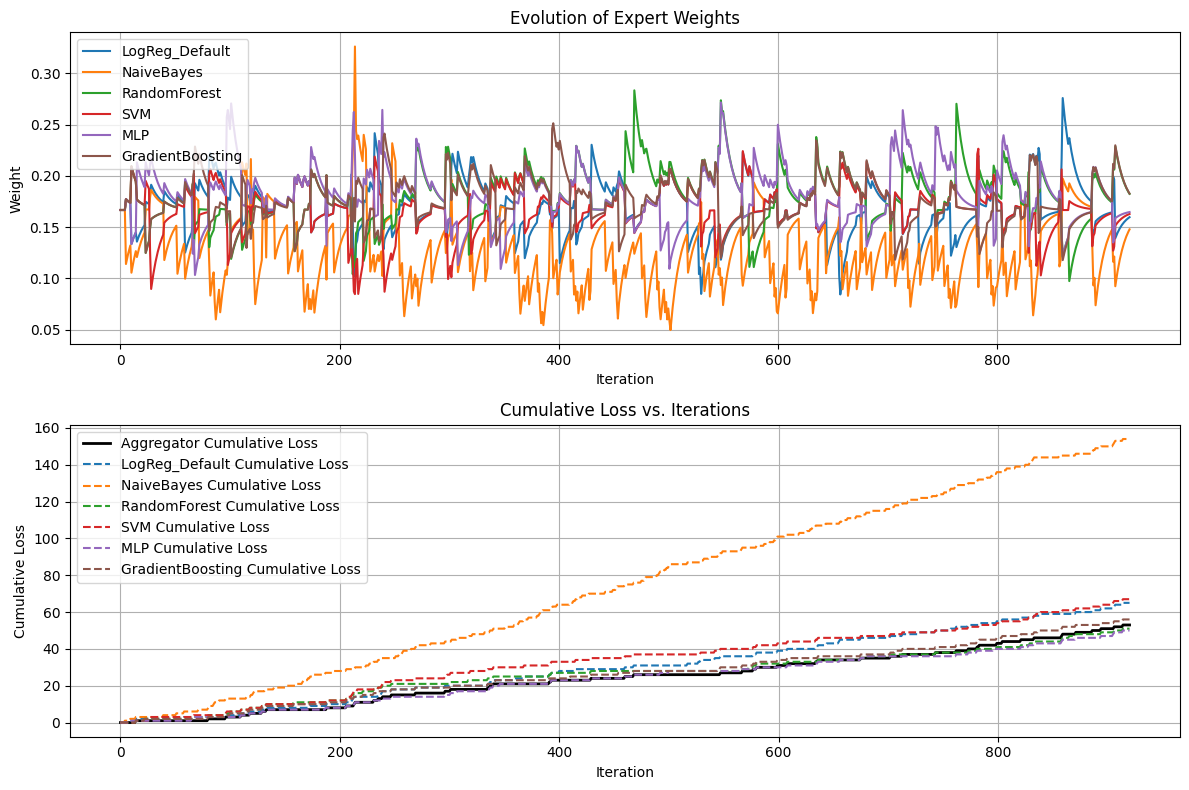
\includegraphics[width=\textwidth]{spambase_fixed_0.1.png}
        \caption{Fixed-Share ($\alpha = 0.1$)}
        \label{fig:supervised_fixed_share_weights_0.1}
      \end{subfigure}
      \begin{subfigure}[b]{0.3\textwidth}
        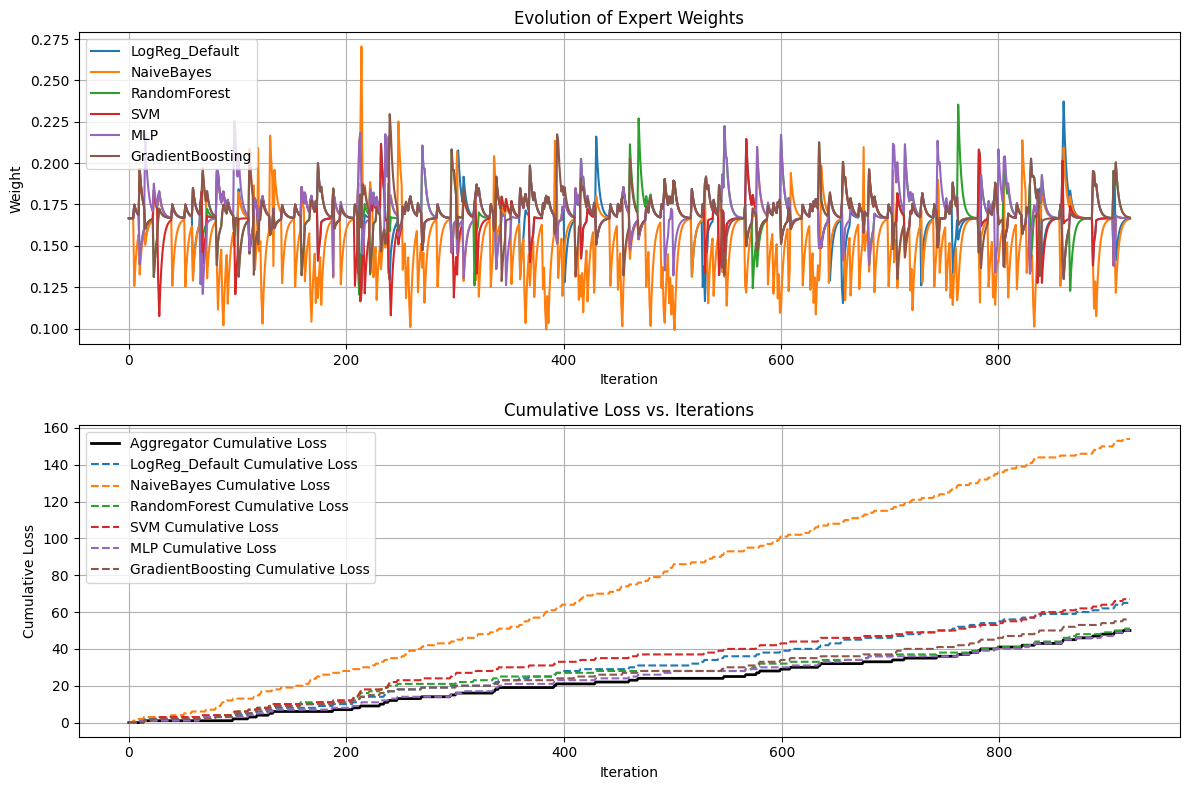
\includegraphics[width=\textwidth]{spambase_fixed_0.3.png}
        \caption{Fixed-Share ($\alpha = 0.3$)}
        \label{fig:supervised_fixed_share_weights_0.3}
      \end{subfigure}
      \caption{Evolution of expert weights and cummulative loss on the Spambase dataset.}
      \label{fig:supervised_comparison}
    \end{figure}
    \begin{figure}[ht]
      \centering
      \begin{subfigure}[b]{0.3\textwidth}
        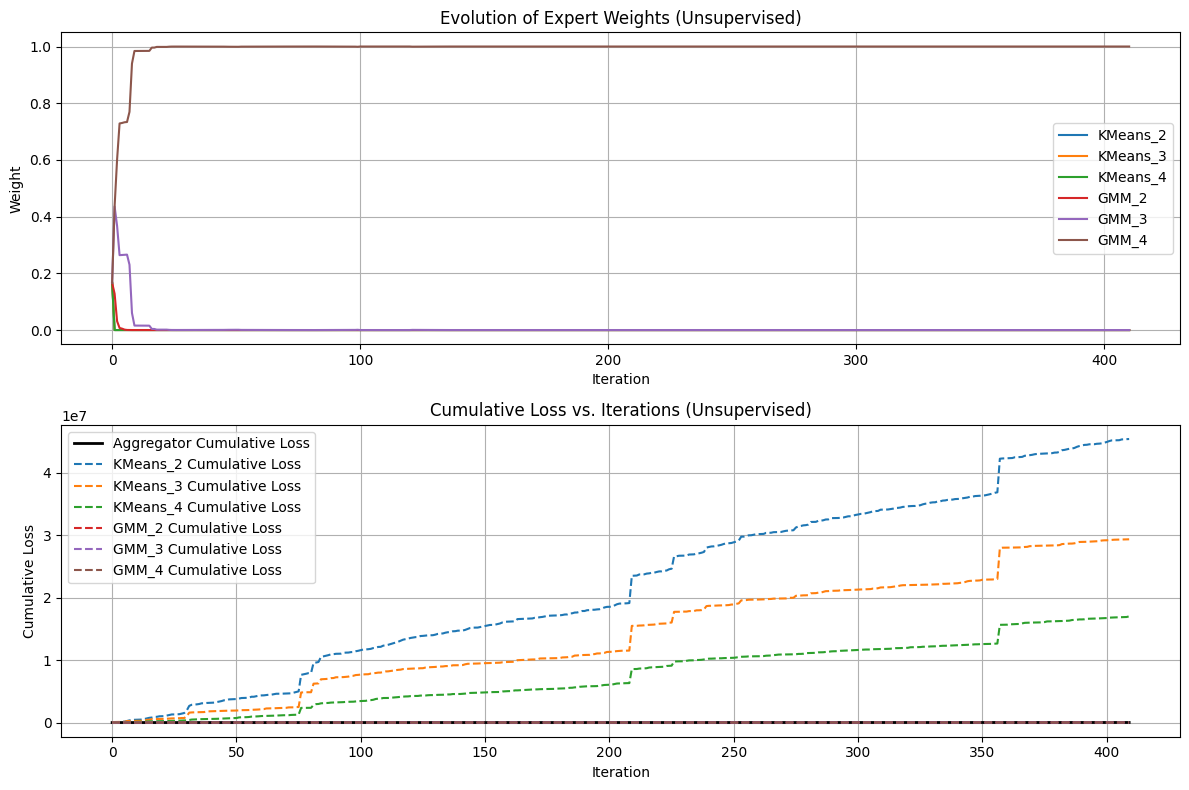
\includegraphics[width=\textwidth]{cloud_static.png}
        \caption{Static Expert}
        \label{fig:unsupervised_static_weights}
      \end{subfigure}
      \begin{subfigure}[b]{0.3\textwidth}
        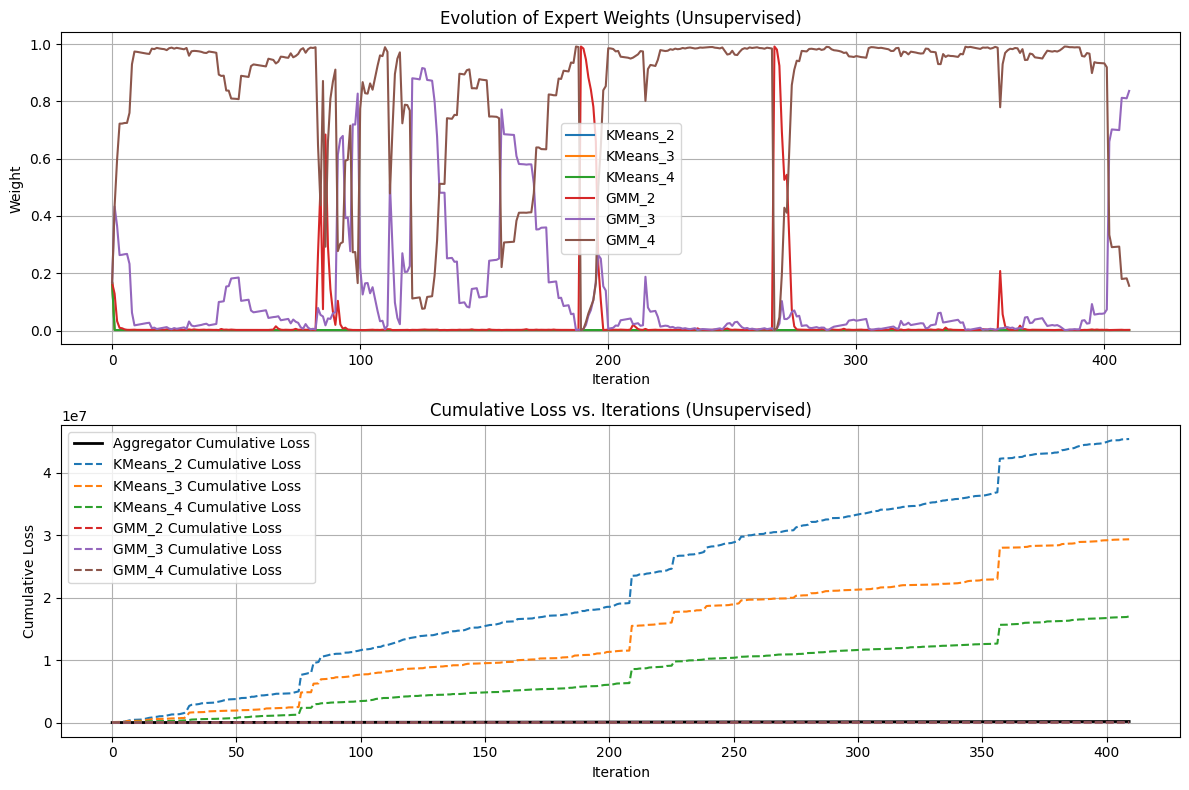
\includegraphics[width=\textwidth]{cloud_fixed_0.01.png}
        \caption{Fixed-Share ($\alpha = 0.01$)}
        \label{fig:unsupervised_fixed_share_weights_0.01}
      \end{subfigure}
      \\
      \begin{subfigure}[b]{0.3\textwidth}
        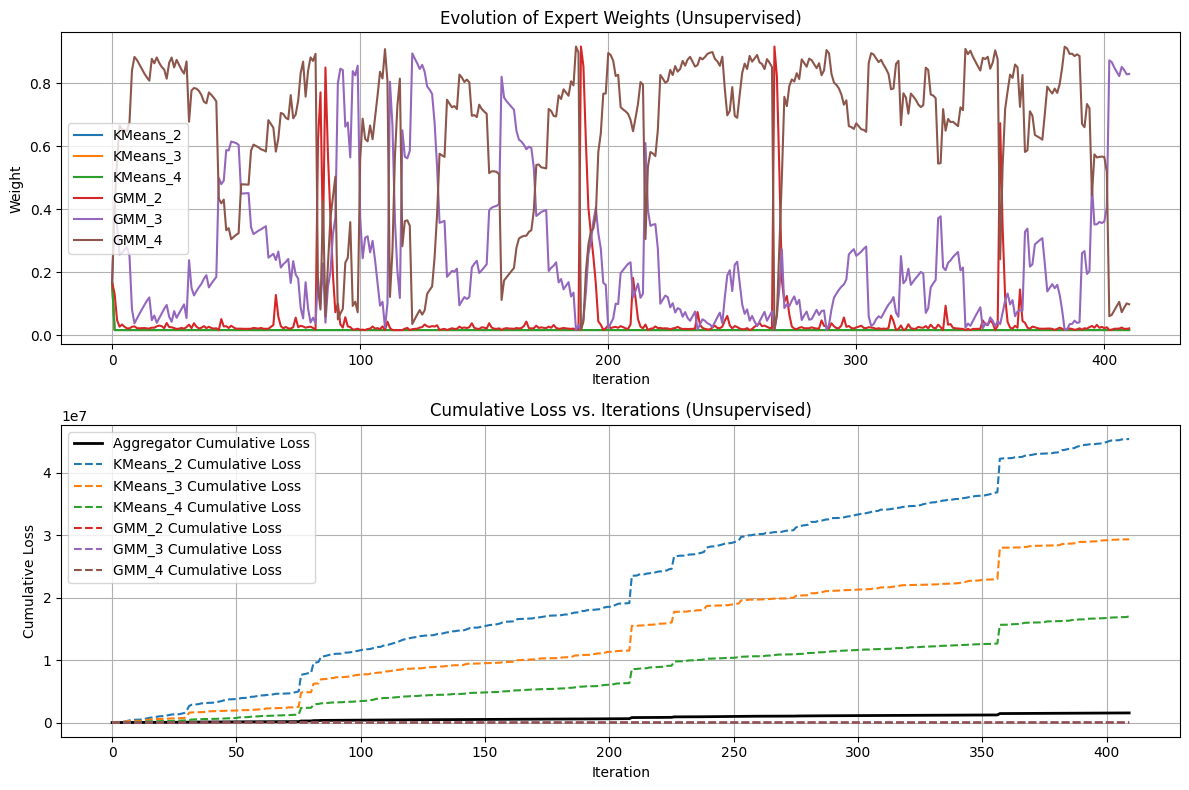
\includegraphics[width=\textwidth]{cloud_fixed_0.1.png}
        \caption{Fixed-Share ($\alpha = 0.1$)}
        \label{fig:unsupervised_fixed_share_weights_0.1}
      \end{subfigure}
      \begin{subfigure}[b]{0.3\textwidth}
        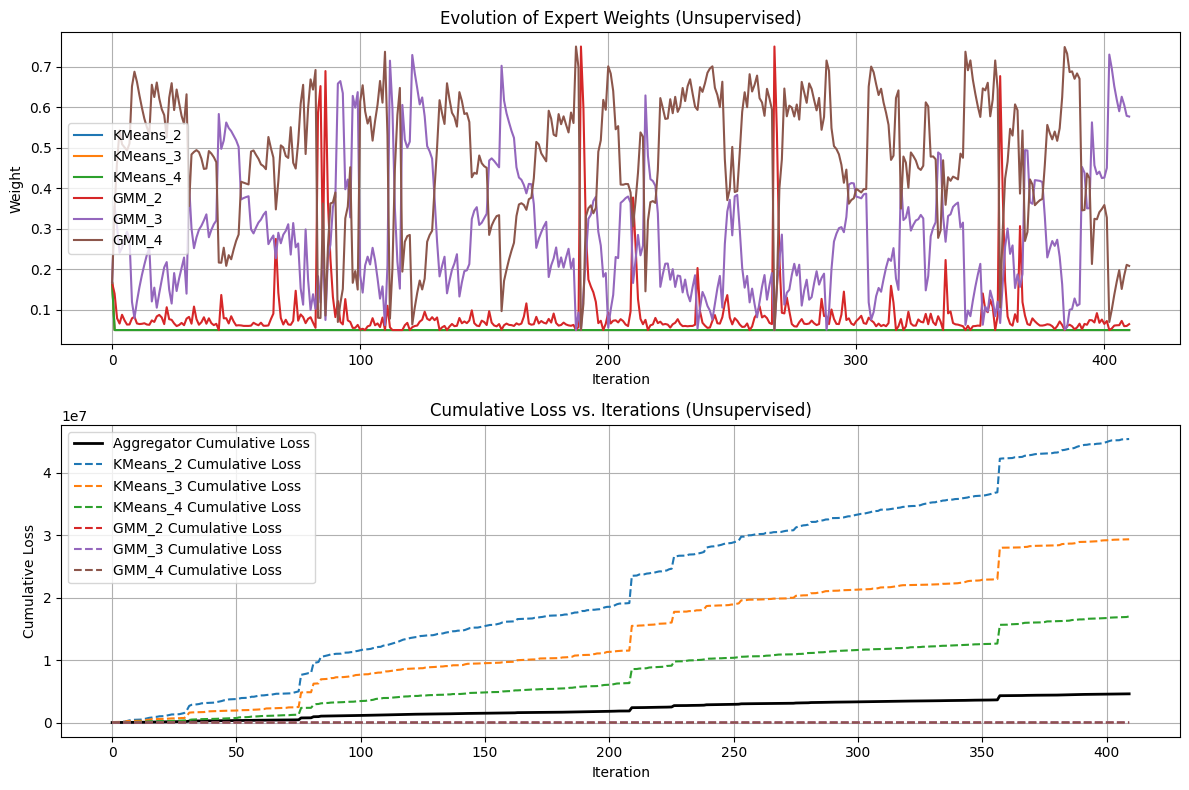
\includegraphics[width=\textwidth]{cloud_fixed_0.3.png}
        \caption{Fixed-Share ($\alpha = 0.3$)}
        \label{fig:unsupervised_fixed_share_weights_0.3}
      \end{subfigure}
      \caption{Evolution of expert weights and cummulative loss on the Cloud dataset.}
      \label{fig:unsupervised_comparison}
    \end{figure}

\subsection*{Conclusions}
In both supervised and unsupervised experiments, the static expert algorithm excels in stable environments where one expert consistently outperforms the others. However, the evolution of weights is influenced by expert diversity: in the supervised setting, more diverse experts cause weights to fluctuate more frequently, while in the unsupervised case, similar experts yield more stable weights. In both scenarios, static aggregation tends to lock in early winners and may struggle to adapt when conditions change.

In contrast, fixed‐share aggregation continuously redistributes weight among experts, enabling rapid recovery if the best performer shifts. The trade-off is that a higher sharing parameter ($\alpha$) improves adaptability but can also introduce increased volatility in stable conditions. Ultimately, selecting an appropriate $\alpha$ hinges on the expected level of nonstationarity in the data.

We can also see that the both weight assignment strategies produce valid results as some experts perform better than others. One such example is the performance of the Naive Bayes classifier in the supervised setting, which consistently underperforms compared to other experts. This is likely due to the independence assumption of the Naive Bayes model, which may not hold in practice. In the unsupervised setting, the Gaussian Mixture Model with 4 components performs well on the Cloud dataset consistently, indicating that it captures the underlying structure effectively.

Therefore, the choice between static and fixed-share aggregation depends on the nature of the problem: static aggregation is suitable for stable environments, while fixed-share aggregation is more robust to nonstationarity. Furthermore, choosing an appropriate $\alpha$ value is crucial for balancing adaptability and stability in the face of changing conditions.

\newpage
\section*{Problem 2}

We want an online update rule
\[
  w_{t+1}
  \;=\;
  \arg\min_{w}
  \Bigl[
    d\bigl(w,w_{t}\bigr)
    \;+\;
    \eta\,L\bigl(y_t,\;w^\top x_t\bigr)
  \Bigr],
\]
where:
\begin{itemize}
\item $L\bigl(y_t, w^\top x_t\bigr)$ is the loss for predicting $w^\top x_t$ when the true label is $y_t$.
\item $\eta>0$ is the learning rate.
\item $d(\cdot,\cdot)$ is a divergence measuring how far $w$ is from $w_t$ (the old parameter vector).
\end{itemize}
Different choices of $d(\cdot,\cdot)$ yield different algorithms:

\subsection*{1. Gradient Descent (GD)}

\paragraph{Distance function:} 
\[
  d\bigl(w, w_t\bigr) 
  \;=\;
  \tfrac12\,\|\,w - w_t\,\|^2.
\]
The update rule becomes
\[
  w_{t+1}
  \;=\;
  \arg\min_{w} 
  \Bigl[
    \tfrac12\,\|\,w - w_t\,\|^2
    \;+\;
    \eta\,L\bigl(y_t, w^\top x_t\bigr)
  \Bigr].
\]

\paragraph{Derivation:}
Define
\[
  \Phi(w)
  \;=\;
  \tfrac12\,\|\,w - w_t\,\|^2
  \;+\;
  \eta\,L\bigl(y_t,\;w^\top x_t\bigr).
\]
Taking its gradient and setting to zero:
\[
  \nabla_{w}\,\Phi(w)
  \;=\;
  (w - w_t)
  \;+\;
  \eta\,\nabla_{w}\,L\bigl(y_t,\;w^\top x_t\bigr)
  \;=\;0.
\]
Hence,
\[
  w
  \;=\;
  w_t
  \;-\;
  \eta\,\nabla_{w}\,L\bigl(y_t,\;w^\top x_t\bigr).
\]
Evaluating the gradient at $w = w_t$ (the typical online update) gives
\[
  \boxed{
    w_{t+1}
    \;=\;
    w_{t}
    \;-\;
    \eta\,\nabla_{w}\,L\Bigl(y_t,\,w_t^\top x_t\Bigr).
  }
\]

\paragraph{Example (Squared Loss):}
If $L(y,\hat{y}) = (y-\hat{y})^2$, then 
$\nabla_{w}\,L = 2(\hat{y}-y)\,x_t$, and 
\[
  w_{t+1}
  \;=\;
  w_t
  \;-\;
  2\,\eta\,\bigl(w_t^\top x_t - y_t\bigr)\,x_t.
\]

\subsection*{2. Exponentiated Gradient (EG)}

\paragraph{Distance function:}
\[
  d\bigl(w,w_t\bigr)
  \;=\;
  \sum_{i} w_i \ln\!\Bigl(\tfrac{w_i}{w_{t,i}}\Bigr),
\]
which is the KL--divergence (assuming $w,\,w_t$ lie in the simplex $\{w:\,\sum_i w_i=1,\;w_i\ge0\}$).

Thus,
\[
  w_{t+1}
  \;=\;
  \arg\min_{\substack{w:\sum_i w_i=1\\w_i\ge0}} 
  \Bigl[
    \sum_{i} w_i \ln\!\Bigl(\tfrac{w_i}{w_{t,i}}\Bigr)
    \;+\;
    \eta\,L\bigl(y_t,\;w^\top x_t\bigr)
  \Bigr].
\]

\paragraph{Derivation (Lagrange multipliers):}
We form
\[
  \mathcal{L}(w,\lambda)
  \;=\;
  \sum_{i}\,
    w_i \ln\!\Bigl(\tfrac{w_i}{\,w_{t,i}\!}\Bigr)
  \;+\;
  \eta\,L\bigl(y_t,\;w^\top x_t\bigr)
  \;+\;
  \lambda\,\Bigl(\sum_{i} w_i - 1\Bigr).
\]
Differentiating w.r.t.\ $w_i$ and setting to zero:
\[
  \frac{\partial \mathcal{L}}{\partial w_i}
  \;=\;
  \ln\!\Bigl(\tfrac{w_i}{w_{t,i}}\Bigr)
  \;+\;
  1
  \;+\;
  \eta \,\bigl[\nabla_w\,L\bigl(y_t,\;w^\top x_t\bigr)\bigr]_i
  \;+\;
  \lambda 
  \;=\;0.
\]
Thus,
\[
  \ln\!\Bigl(\tfrac{w_i}{\,w_{t,i}\!}\Bigr)
  \;=\;
  -\,1 \;-\;\lambda
  \;-\;\eta\,\bigl[\nabla_w\,L\bigr]_i,
\]
so
\[
  w_i
  \;=\;
  e^{-1-\lambda}
  \,\times\,
  w_{t,i}
  \,\exp\!\Bigl(-\,\eta\,\bigl[\nabla_w\,L\bigr]_i\Bigr).
\]
Impose $\sum_i w_i=1$ to solve for $e^{-1-\lambda}$, yielding
\[
  \boxed{
  w_{t+1,i}
  \;=\;
  \frac{
    w_{t,i}\,\exp\!\Bigl(-\,\eta\,\bigl[\nabla_w\,L\bigr]_i\Bigr)
  }{
    \sum_{j}\,
      w_{t,j}\,\exp\!\Bigl(-\,\eta\,\bigl[\nabla_w\,L\bigr]_j\Bigr)
  }.
  }
\]

\section*{Problem 3}

We have the following classes with their respective distances from the margin $h$ as follows:
\begin{enumerate}
    \item Red: 1.5, 1.5, 2, 3, 4
    \item Blue: 1, 1, 2, 6
    \item Green: 2, 6, 7
    \item Orange: 2, 3, 6, 8
\end{enumerate}
with a total of 16 points.\\

\noindent We can calculate the class conditional means as follows:
\begin{align}
    E[h(x) | y_{\text{red}}] &= \frac{1.5 + 1.5 + 2 + 3 + 4}{5} = 2.4\\
    E[h(x) | y_{\text{blue}}] &= \frac{1 + 1 + 2 + 6}{4} = 2.5\\
    E[h(x) | y_{\text{green}}] &= \frac{2 + 6 + 7}{3} = 5\\
    E[h(x) | y_{\text{orange}}] &= \frac{2 + 3 + 6 + 8}{4} = 4.75
\end{align}
The overall mean is 
\begin{align}
    E[h(x)] &= \frac{\text{Red}(12) + \text{Blue}(10)+ \text{Green}(15) + \text{Orange}(19)}{16} = \frac{56}{16} = 3.5
\end{align}
The absolute deviation of each class from the overall mean is as follows:
\begin{align}
    |E[h(x)] - E[h(x) | y_{\text{red}}]| &= |3.5 - 2.4| = 1.1\\
    |E[h(x)] - E[h(x) | y_{\text{blue}}]| &= |3.5 - 2.5| = 1\\
    |E[h(x)] - E[h(x) | y_{\text{green}}]| &= |3.5 - 5.0| =1.5\\
    |E[h(x)] - E[h(x) | y_{\text{orange}}]| &= |3.5 - 4.75| = 1.25
\end{align}
Average across all classes is:
\begin{align}
    E_y[|E[h(x)] - E[h(x) | y]|] &= \frac{1.1 + 1 + 1.5 + 1.25}{4} = 1.2125
\end{align}
The objective function is given by:
\begin{align}
    J(h) &= \frac{1}{2}E_y[|E[h(x)] - E[h(x) | y]|]\\
    &= \frac{1}{2} \times 1.2125 = 0.60625
\end{align}

\newpage
\section*{Problem 4}

\subsection*{i. Supervised Settings}

\begin{figure}[ht]
    \centering
    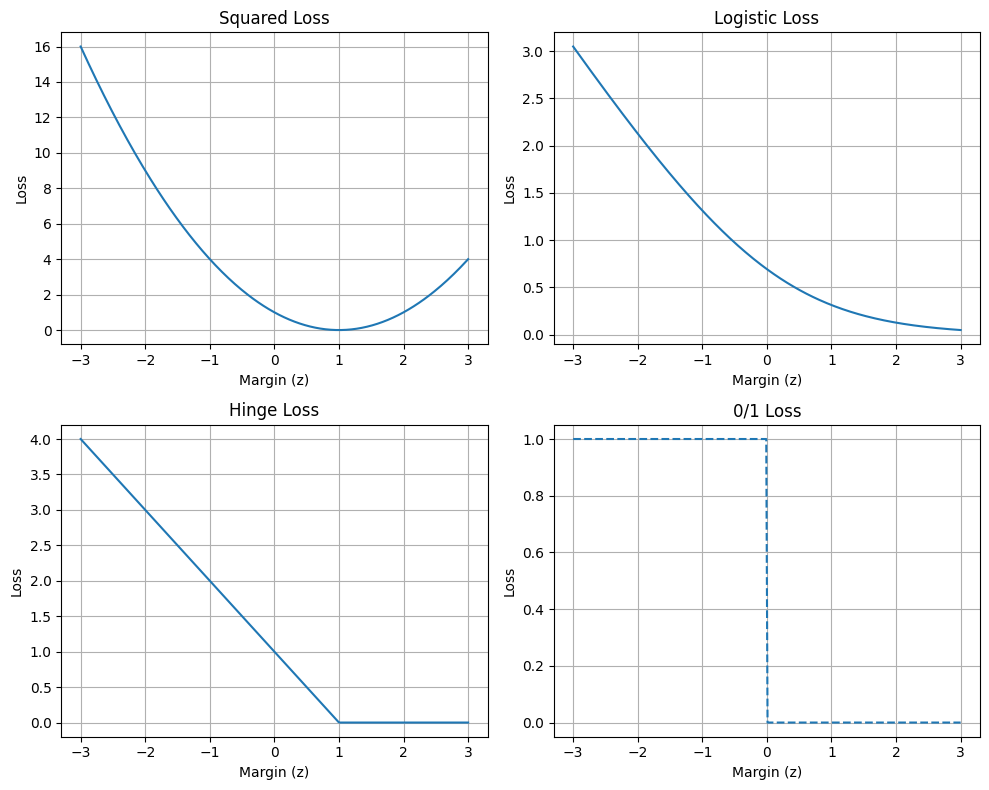
\includegraphics[width=0.6\textwidth]{loss.png}
    \caption{Comparison of different loss functions.}
    \label{fig:losses}
    
\end{figure}

\begin{enumerate}
    \item Squared Loss: $(1-z)^2$\\
    Smooth, convex, and quadratic. Penalizes errors heavily; small errors incur small loss but large errors explode. Sensitive to outliers due to quadratic growth.
    \item Logistic Loss: $\ln(1+\exp(-z))$\\
    Smooth, convex, and has probabilistic interpretation. Rapidly decreases for large positive margins, yet remains sensitive to errors near the decision boundary. Provides well-calibrated probabilities; less aggressive than squared loss for extreme errors.
    \item Hinge Loss: $\max(0, 1-z)$\\
    Convex but non-smooth at $z=1$. Applies a linear penalty for margin violations ($z < 1$); zero loss when $z \geq 1$. Focuses only on points near the decision boundary (support vectors), useful in SVMs.
    \item 0-1 Loss: $1 \text{ if } z < 0, \text{ else } 0$\\
    Non-convex and discontinuous. Only distinguishes between correct and incorrect classification without considering the margin. Ideal for evaluation but impractical for direct optimization due to lack of gradient information.
    
\end{enumerate}


\subsection*{ii. Unsupervised Settings}
\subsubsection*{K Nearest Neighbors (KNN) and Outliers}
For this problem, we consider the classic \href{https://archive.ics.uci.edu/dataset/53/iris}{Iris} dataset. The data set contains 3 classes. One class is linearly separable from the other 2; the latter are not linearly separable from each other.\\


We use the \texttt{KMeans} from \texttt{sklearn} to cluster the data into $K=3$ clusters. To plot the clusters in 2D, we apply PCA. The results are shown in Figure \ref{fig:kmeans}.
\begin{figure}[ht]
    \centering
    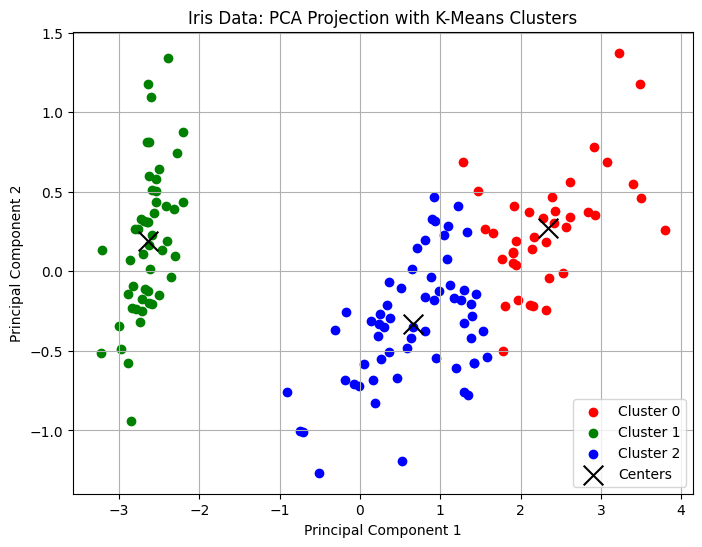
\includegraphics[width=0.6\textwidth]{knn-iris.png}
    \caption{KMeans clustering of the Iris dataset.}
    \label{fig:kmeans}
\end{figure}
As per the the description of the dataset, the \texttt{green} class is linearly separable from the \texttt{red} and \texttt{blue} classes but they are not linearly separable from each other.
\newpage
\noindent The costs of the clustering are as follows:
\begin{enumerate}
    \itemsep 0em
    \item K-means cost (sum squared distances): 63.82
    \item K-median cost (sum absolute distances): 104.84
    \item K-center cost (max distance): 1.63
\end{enumerate}
We then introduce 3 outliers to the dataset:
\[
\{
    (8,8), (-8,-8), (8, -8)
\}
\]
\begin{figure}[ht]
    \centering
    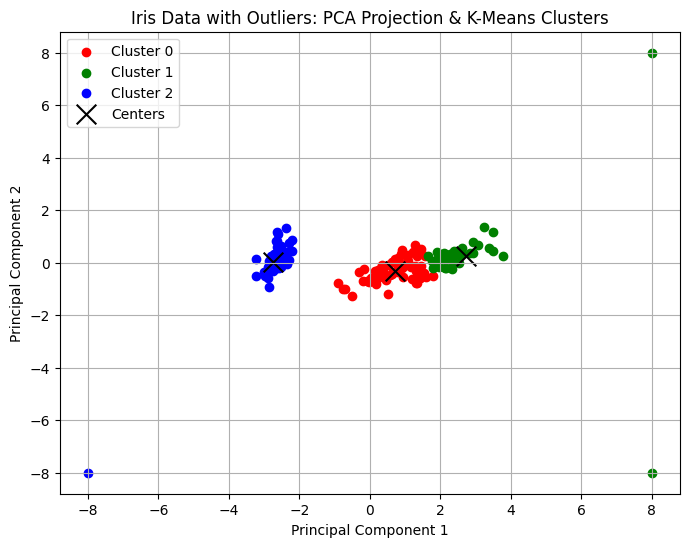
\includegraphics[width=0.6\textwidth]{knn-iris-out.png}
    \caption{KMeans clustering of the Iris dataset with outliers.}
    \label{fig:kmeans-outliers}
\end{figure}
\newpage
\noindent Re-running the KMeans clustering, the costs of the clustering with outliers are as follows:
\begin{enumerate}
    \itemsep 0em
    \item K-means cost (sum squared distances): 345.29
    \item K-median cost (sum absolute distances): 152.69
    \item K-center cost (max distance): 9.79
\end{enumerate}
Each cost metric responds differently to the presence of outliers:
\begin{itemize}
\item {K-means Cost (Sum of Squared Distances)}
\[
J_{\text{K-means}} = \sum_{i=1}^{n} \| x_i - \mu_{c(i)} \|^2.
\]
Because the error is squared, even moderate deviations are amplified. In our example, the cost increases from 63.82 to 345.29—a 440\% increase—illustrating how outliers with large deviations disproportionately affect the overall cost.

\item {K-median Cost (Sum of Absolute Distances)}
\[
J_{\text{K-median}} = \sum_{i=1}^{n} \| x_i - \mu_{c(i)} \|_1.
\]
Here, errors are penalized linearly. Thus, while outliers do increase the cost, their impact is less dramatic. The cost increases from 104.84 to 152.69 (a 45\% increase), reflecting a moderate sensitivity to outliers.

\item {K-center Cost (Maximum Distance)}
\[
J_{\text{K-center}} = \max_{1 \leq i \leq n} \| x_i - \mu_{c(i)} \|.
\]
This metric depends solely on the farthest (worst-case) point. A single outlier with a large deviation can cause a significant increase. Here, the cost jumps from 1.63 to 9.79—a 500\% increase—demonstrating extreme sensitivity to outliers.
\end{itemize}

\newpage
\subsection*{K-means Clustering and Initialization}
For this part, we initialize data using four 2D gaussian random variables with the following parameters:
\begin{align*}
    \mu_1 &= (0, 0), \quad \Sigma_1 = \begin{bmatrix} 0.5 & 0 \\ 0 & 0.5 \end{bmatrix}\qquad\mu_2 = (0, 10), \quad \Sigma_2 = \begin{bmatrix} 0.5 & 0 \\ 0 & 0.5 \end{bmatrix}\\
    \mu_3 &= (10, 0), \quad \Sigma_3 = \begin{bmatrix} 0.5 & 0 \\ 0 & 0.5 \end{bmatrix}\qquad\mu_4 = (10, 10), \quad \Sigma_4 = \begin{bmatrix} 0.5 & 0 \\ 0 & 0.5 \end{bmatrix}
\end{align*}
This ensures that the clusters are well-separated, have equal variance, and fairly concentrated. We then run K-means clustering with 4 clusters and 2 different initialization strategies:
\begin{enumerate}
    \item Initialize with centroids at the true means.
    \item Initialize with centroids such that some means are not covered by any cluster.
\end{enumerate}
The results are shown in Figure \ref{fig:knn-init}.
\begin{figure}[ht]
    \centering
    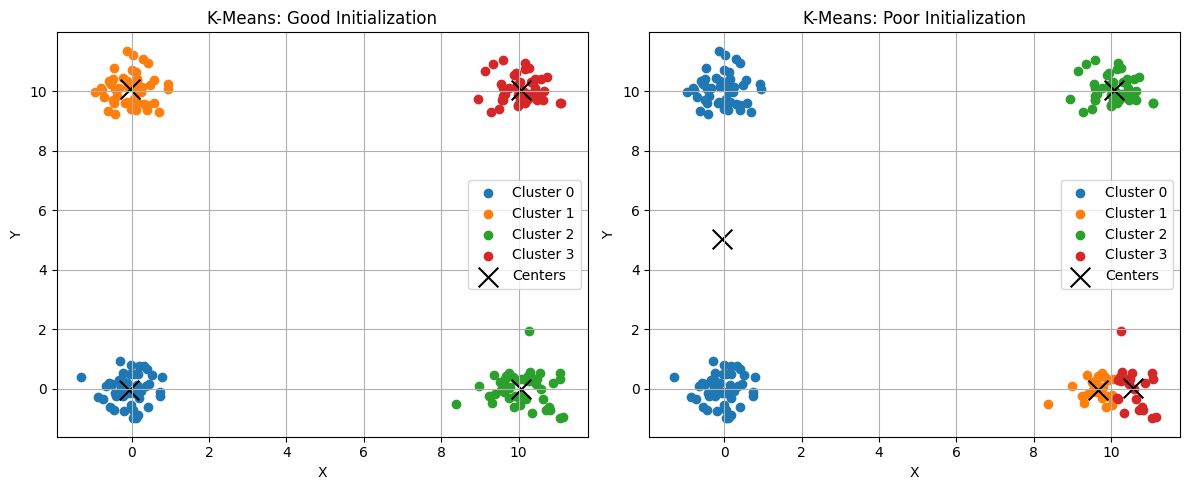
\includegraphics[width=1\textwidth]{knn-gauss.png}
    \caption{KMeans clustering with different initialization strategies.}
    \label{fig:knn-init}
\end{figure}
We observe that the initialization strategy significantly affects the clustering outcome. When initialized with centroids at the true means, the algorithm converges to the correct clusters. However, when initialized such that some means are not covered by any cluster, the algorithm converges to a suboptimal solution, incorrectly merging clusters. This shows that K-means is highly sensitive to initialization.

\section*{Appendix}
\subsection*{Problem 1: Code Implementation}
\includepdf[pages=-]{q1_spambase.pdf}
\includepdf[pages=-]{q1_cloud.pdf}
\subsection*{Problem 4: Code Implementation}
\includepdf[pages=-]{q4.pdf}








\end{document}